\section{moeo\-Easy\-EA$<$ MOEOT $>$::eo\-Dummy\-Transform Class Reference}
\label{classmoeoEasyEA_1_1eoDummyTransform}\index{moeoEasyEA::eoDummyTransform@{moeoEasyEA::eoDummyTransform}}
a dummy transform  


{\tt \#include $<$moeo\-Easy\-EA.h$>$}

Inheritance diagram for moeo\-Easy\-EA$<$ MOEOT $>$::eo\-Dummy\-Transform::\begin{figure}[H]
\begin{center}
\leavevmode
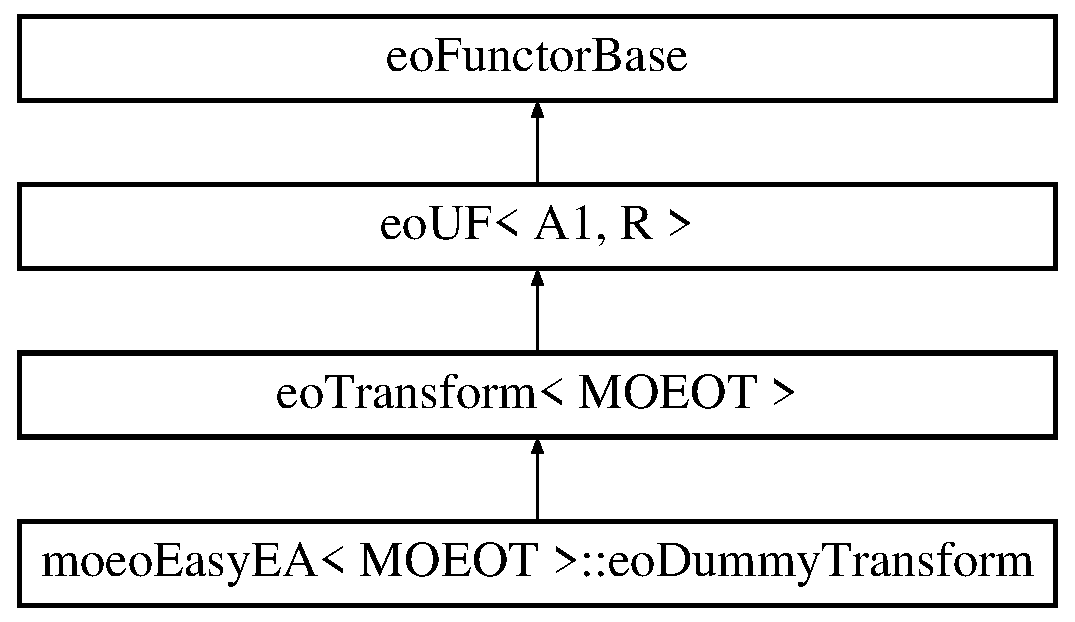
\includegraphics[height=4cm]{classmoeoEasyEA_1_1eoDummyTransform}
\end{center}
\end{figure}
\subsection*{Public Member Functions}
\begin{CompactItemize}
\item 
void \bf{operator()} (\bf{eo\-Pop}$<$ MOEOT $>$ \&)\label{classmoeoEasyEA_1_1eoDummyTransform_0e153e482291a7f19f7f7a02505fb432}

\begin{CompactList}\small\item\em the dummy functor \item\end{CompactList}\end{CompactItemize}


\subsection{Detailed Description}
\subsubsection*{template$<$class MOEOT$>$ class moeo\-Easy\-EA$<$ MOEOT $>$::eo\-Dummy\-Transform}

a dummy transform 



Definition at line 233 of file moeo\-Easy\-EA.h.

The documentation for this class was generated from the following file:\begin{CompactItemize}
\item 
moeo\-Easy\-EA.h\end{CompactItemize}
